% !TEX program = pdflatex
\documentclass[11pt,a4paper]{article}

\usepackage[margin=1in]{geometry}
\usepackage{graphicx}
\usepackage{booktabs}
\usepackage{caption}
\usepackage{subcaption}
\usepackage{xcolor}
\usepackage[hidelinks,colorlinks=true,linkcolor=teal,urlcolor=teal,citecolor=teal]{hyperref}
\usepackage{enumitem}
\usepackage{float}
\usepackage{fancyhdr}
\usepackage{titlesec}
\usepackage{microtype}

% --- Header / footer ---
\pagestyle{fancy}
\fancyhf{}
\fancyhead[L]{\small Human Fetal Heart PCW 11--13 — Data Overview}
\fancyhead[R]{\small \thepage}
\renewcommand{\headrulewidth}{0.4pt}

% --- Section formatting ---
\titleformat{\section}{\Large\bfseries\color{teal!60!black}}{\thesection}{0.6em}{}
\titleformat{\subsection}{\large\bfseries\color{black}}{\thesubsection}{0.5em}{}

% --- Caption styling ---
\captionsetup{font=small,labelfont=bf,labelsep=period}

% --- Figure path ---
\graphicspath{{figures/overview/}}

% ====================================================================
\title{\textbf{Human Fetal Heart PCW 11--13 \\[0.1em] \large Multi-modal Single-cell and Spatial Atlas — Data Overview}}
\author{\textit{PCW12\_analysis project}}
\date{\today}

\begin{document}
\maketitle
\thispagestyle{fancy}

% --- Abstract ---
\begin{abstract}
\noindent
This document summarizes the two human fetal heart datasets that underlie the
\textsf{PCW12\_analysis} project: a 95{,}684-cell scRNA-seq atlas spanning
post-conceptional weeks (PCW) 11--13 across 8 donors, and a 100{,}000-cell
MERFISH 3D spatial transcriptomics dataset of a single PCW-12 specimen
(downsampled from a 1.7M-cell full atlas) with a 238-gene panel and 53 serial
sections. We characterize per-cell quality control, sample composition,
cell-type abundance in both modalities, and the spatial layout of the MERFISH
specimen. A cross-modality comparison shows strong concordance in broad
cell-type proportions, supporting the use of these datasets together for
downstream tasks such as gene imputation and disease-gene spatial mapping.
\end{abstract}

\vspace{0.5em}

% ====================================================================
\section{Datasets}

\begin{table}[H]
\centering
\small
\renewcommand{\arraystretch}{1.15}
\begin{tabular}{@{}p{0.30\textwidth} p{0.30\textwidth} p{0.30\textwidth}@{}}
\toprule
\textbf{Property} & \textbf{scRNA-seq} & \textbf{MERFISH (3D spatial)} \\
\midrule
File & \texttt{all\_healthy\_RoundedPCW11-13.h5ad} & \texttt{full\_heart\_final\_aug2025\_update\_downsampled\_100k.h5ad} \\
Cells & 95{,}684 & 100{,}000 (subsampled from $\sim$1.7M) \\
Genes / panel size & 31{,}019 (full transcriptome) & 238 (targeted MERFISH panel) \\
Developmental stage & PCW 11, 12, 13 & PCW 12 \\
Donors / specimens & 8 donors, 24 samples & 1 specimen, 53 serial sections \\
Modality batches & --- & 2 (ATR: atrial, VEN: ventricular) \\
Cell-type annotations & 11 broad / 111 fine & 34 fine \\
Layers & \texttt{counts} (raw) & \texttt{counts} (raw); X is log1p \\
Embeddings shipped & --- & \texttt{X\_pca}, \texttt{X\_pca\_harmony}, \texttt{X\_umap}, \texttt{X\_spatial} (2D), \texttt{X\_spateo\_update} (3D) \\
\bottomrule
\end{tabular}
\caption{High-level summary of the two h5ad inputs used in this project.}
\label{tab:datasets}
\end{table}

\noindent
The scRNA-seq atlas is multi-donor and spans PCW 11--13 to provide a
transcriptomic reference, while the MERFISH dataset provides spatial
context for a single PCW-12 heart at near-cellular resolution across the
whole organ. Per-cell quality metrics (UMI counts, genes detected,
mitochondrial fraction, cell volume) and standard metadata (sex, donor,
cell-cycle phase, FOV, section) are pre-computed in the AnnData
\texttt{obs} fields and used directly in the figures below.

% ====================================================================
\section{scRNA-seq quality and composition}

\subsection{Per-cell QC metrics}

\begin{figure}[H]
\centering
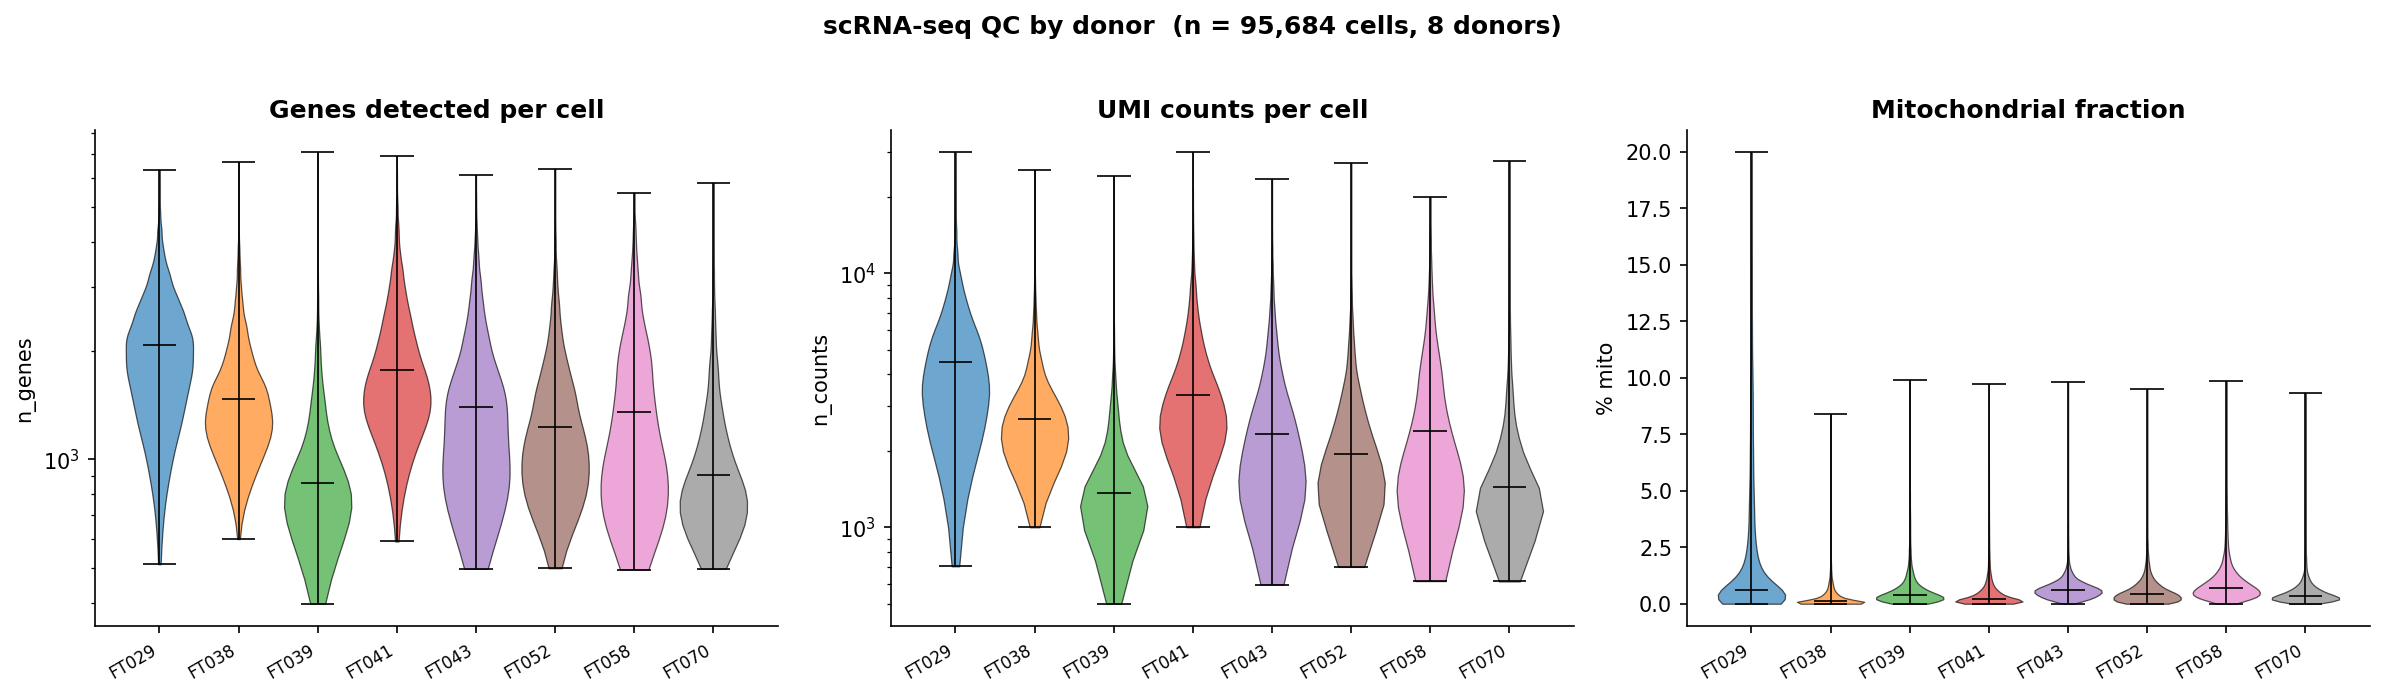
\includegraphics[width=\textwidth]{scrna_qc.png}
\caption{Per-cell QC distributions for the scRNA-seq atlas, split by donor
(\(n=8\) donors). Median values across all 95{,}684 cells:
\textbf{1{,}375} genes per cell, \textbf{2{,}389} UMI counts per cell, and
\textbf{0.41\%} mitochondrial content. Donor FT029 has a longer mitochondrial
tail, but the bulk of cells in every donor sit below 5\% — well within accepted
thresholds for fetal tissue scRNA-seq. The log-scaled \(n\)\textunderscore counts
panel shows comparable depth across donors except for FT039 and FT070, which
are slightly shallower; this is consistent with their smaller cell counts.}
\label{fig:scrna_qc}
\end{figure}

\subsection{Cell-type composition}

\begin{figure}[H]
\centering
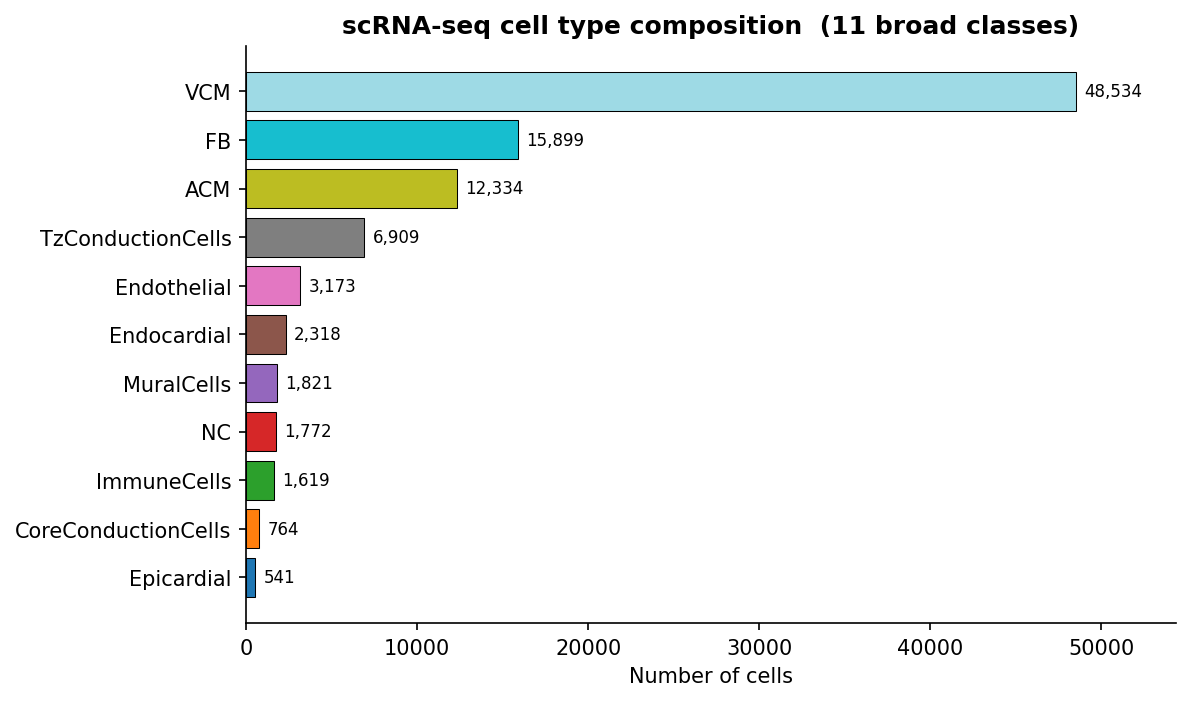
\includegraphics[width=0.85\textwidth]{scrna_celltype.png}
\caption{Cell counts per broad cell-type label (\(\textsf{celltype\_label}\),
11 classes). Ventricular cardiomyocytes (\textbf{VCM}, 50.7\%) dominate the
atlas, followed by fibroblasts (\textbf{FB}, 16.6\%) and atrial cardiomyocytes
(\textbf{ACM}, 12.9\%). Conduction-system, endothelial, endocardial, mural,
neural-crest, immune and epicardial populations together account for the
remaining 19.8\% — an expected composition for a fetal cardiac atlas.
A fine-grained label (\(\textsf{celltype}\), 111 classes) is also available
for more granular analyses.}
\label{fig:scrna_celltype}
\end{figure}

\subsection{Donors, developmental stage, sex, and cell cycle}

\begin{figure}[H]
\centering
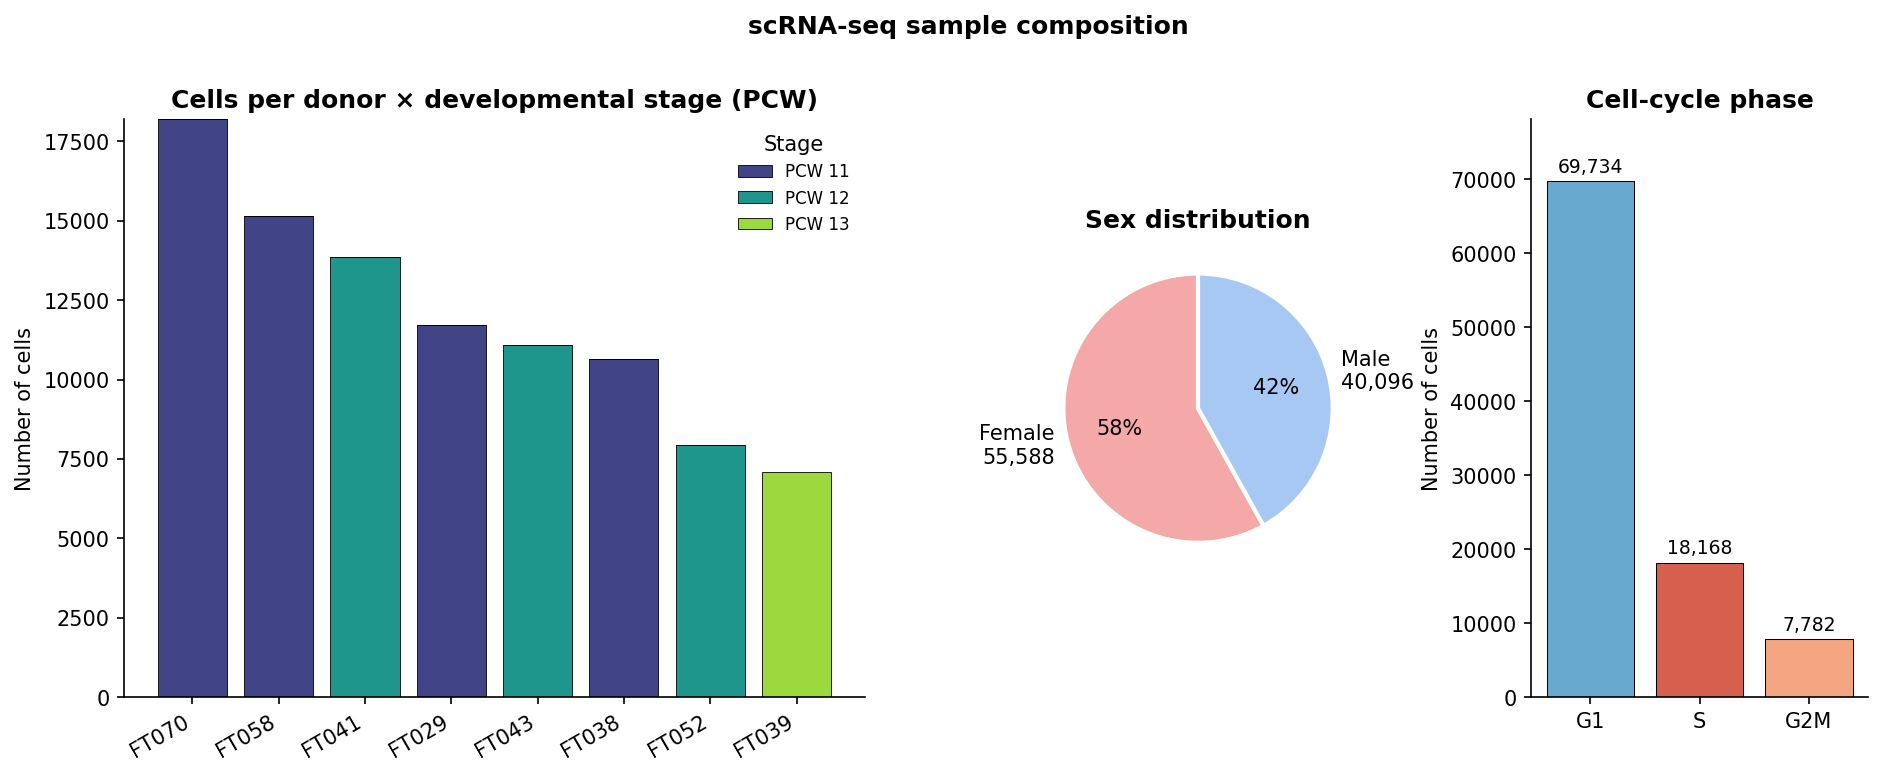
\includegraphics[width=\textwidth]{scrna_donor_pcw.png}
\caption{Sample composition. \textbf{Left:} cells per donor coloured by
developmental stage (PCW). Each donor was sampled at a single PCW: FT029,
FT041, FT043, FT052 at PCW 12; FT038, FT058, FT070 at PCW 11; FT039 at
PCW 13. PCW-11 cells dominate the atlas (55{,}730 cells, 58\%) followed by
PCW 12 (32{,}870, 34\%) and PCW 13 (7{,}084, 7\%).
\textbf{Centre:} sex distribution (58\% female, 42\% male).
\textbf{Right:} cell-cycle phase scoring — \(\sim\)27\% of cells are in
S or G2/M, consistent with the high proliferative activity expected during
mid-gestation cardiogenesis.}
\label{fig:scrna_donor}
\end{figure}

% ====================================================================
\section{MERFISH quality and composition}

\subsection{Per-cell QC metrics}

\begin{figure}[H]
\centering
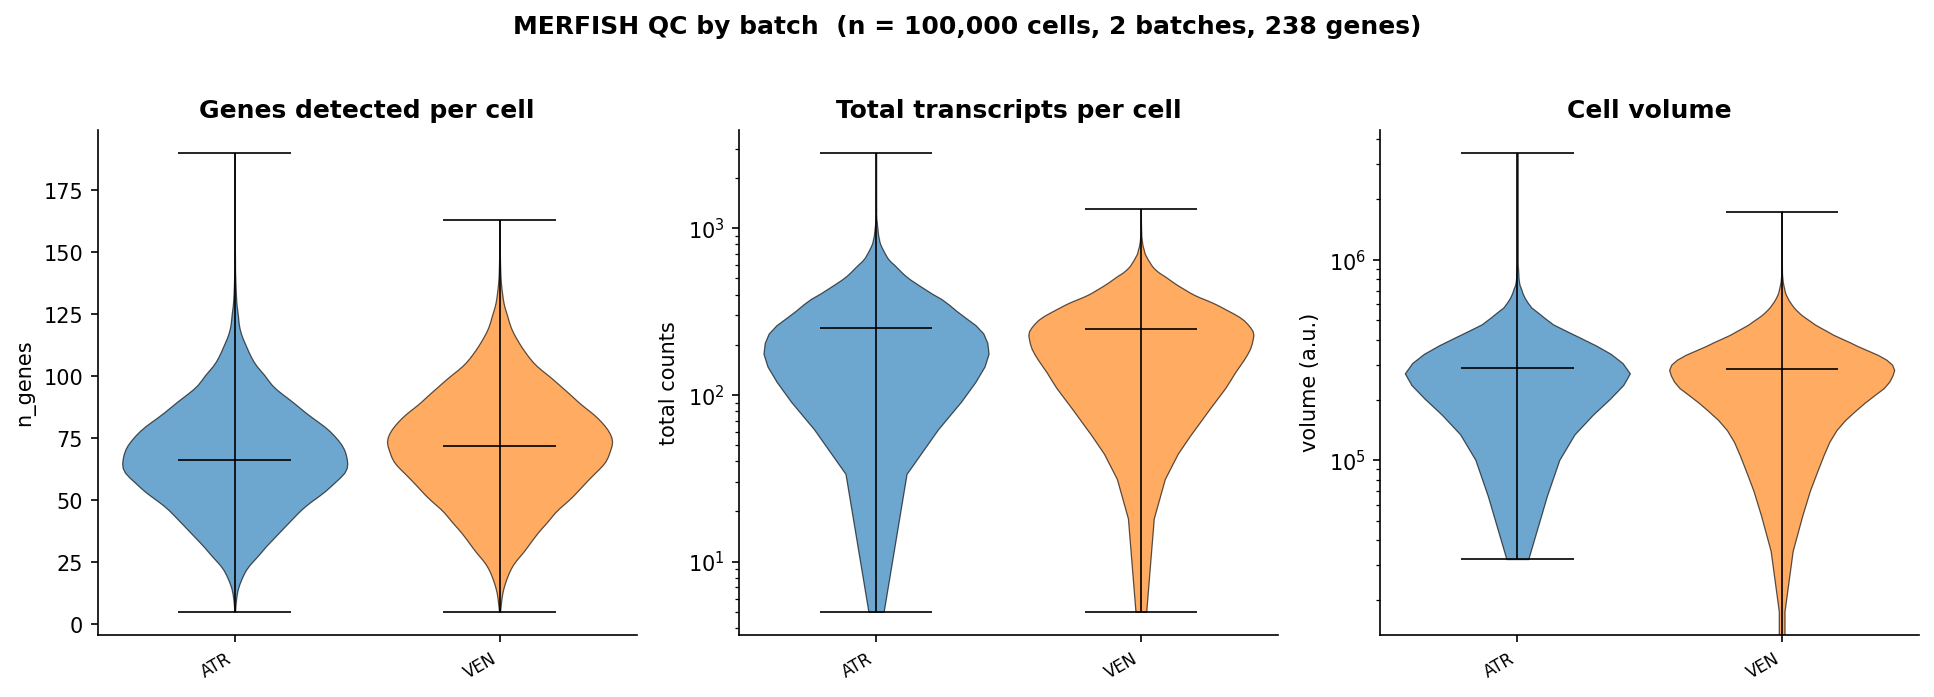
\includegraphics[width=\textwidth]{merfish_qc.png}
\caption{MERFISH per-cell QC, split by batch (ATR = atrial-region sections,
VEN = ventricular-region sections). Median values: \textbf{69} genes detected
per cell out of the 238-gene panel, \textbf{251} total transcripts per cell,
and a cell volume of \textbf{2.86\(\times\)10\(^{5}\)}\,a.u. The two batches
have nearly identical distributions across all three metrics, indicating that
batch effects on per-cell yield are minimal. The log-scale total-counts
panel reveals a small low-yield tail in both batches that may benefit from
filtering for sensitive downstream analyses.}
\label{fig:merfish_qc}
\end{figure}

\subsection{Cell-type composition}

\begin{figure}[H]
\centering
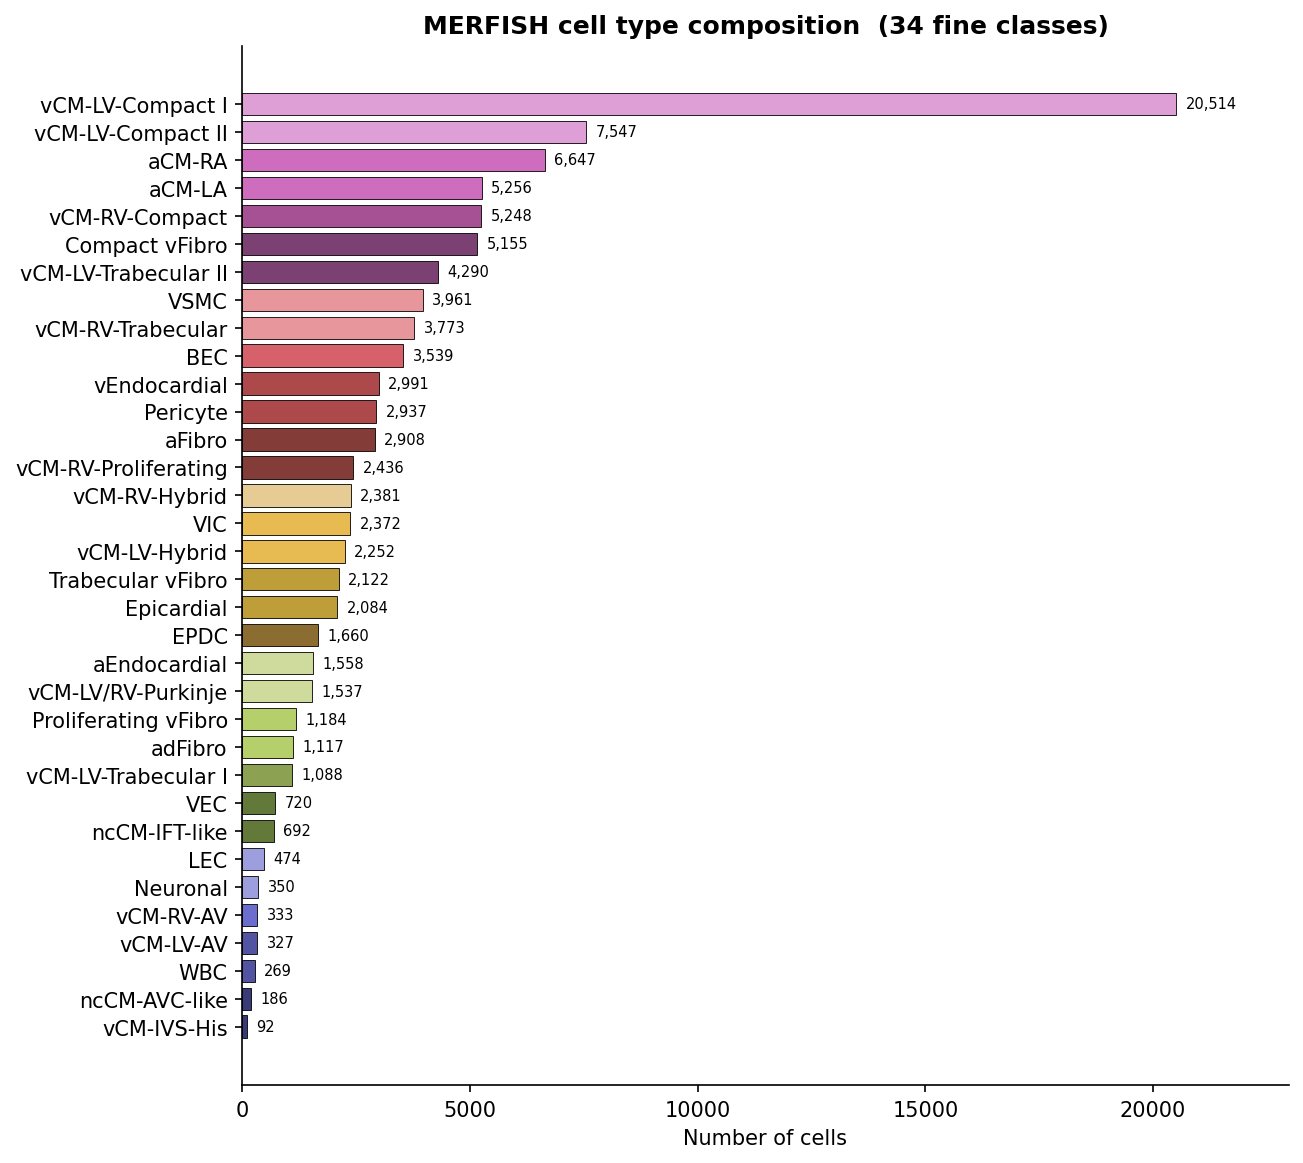
\includegraphics[width=0.85\textwidth]{merfish_celltype.png}
\caption{MERFISH cell-type composition (34 fine classes, ranked by
abundance). The most abundant population is \textsf{vCM-LV-Compact I}
(20{,}514 cells, 20.5\%), reflecting the size of the compact left
ventricular myocardium at PCW 12. Most rare populations
(WBC, ncCM-AVC-like, vCM-IVS-His) still have $\geq$90 cells, providing
sufficient sample sizes for cell-type-level spatial analysis.}
\label{fig:merfish_celltype}
\end{figure}

\subsection{Sectioning and field-of-view structure}

\begin{figure}[H]
\centering
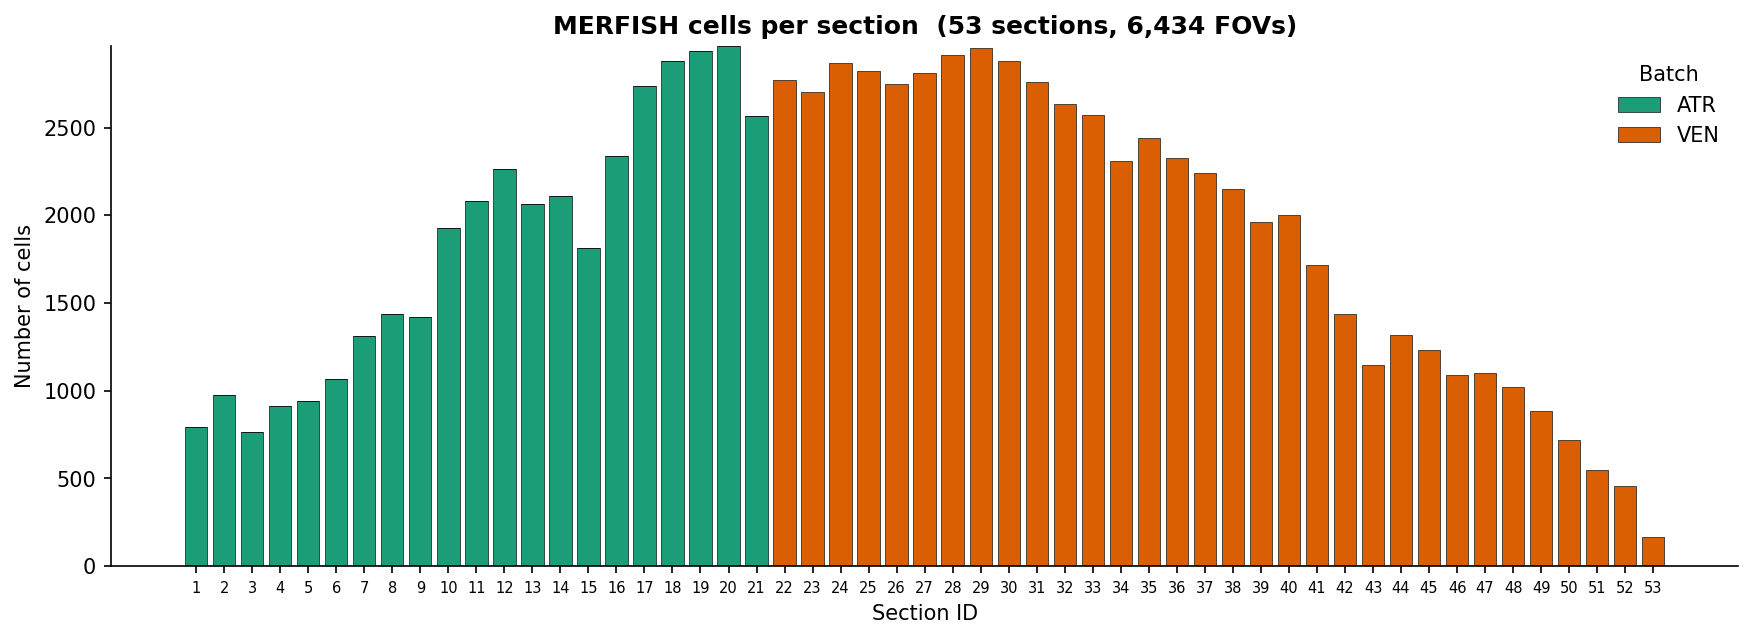
\includegraphics[width=\textwidth]{merfish_section.png}
\caption{Cells per serial section (53 sections total, organized into 6{,}434
fields of view across two batches). Sections 1--21 (\textbf{ATR}, green)
cover atrial regions; sections 22--53 (\textbf{VEN}, orange) cover the
ventricles. The roughly bell-shaped yield within each batch reflects the
varying physical cross-section of the developing heart along the axial
direction — central sections capture the largest tissue area and therefore
the most cells.}
\label{fig:merfish_section}
\end{figure}

\subsection{2D anatomical layout}

\begin{figure}[H]
\centering
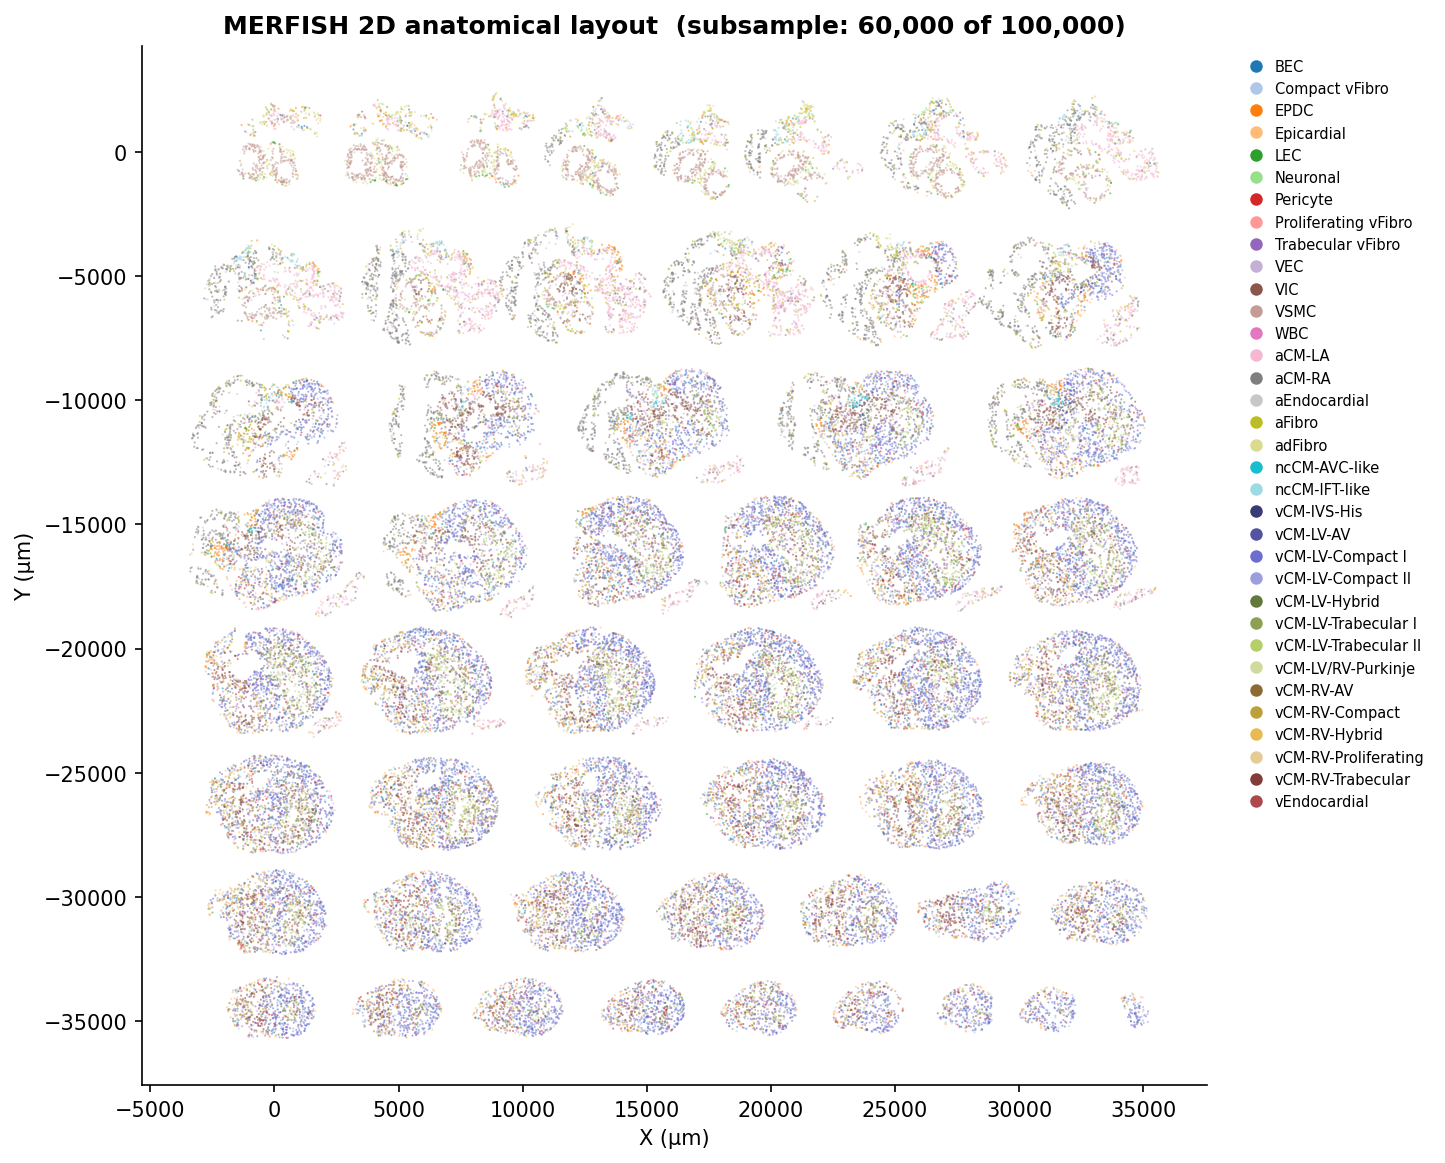
\includegraphics[width=0.95\textwidth]{merfish_spatial.png}
\caption{2D arrangement of all 53 serial sections in the
\(\textsf{X\_spatial}\) embedding, coloured by the 34-class fine cell type.
Each ``island'' is one anatomical section. The atrial sections (top rows) are
smaller and morphologically distinct from the ventricular sections (bottom
rows), with progressively larger cross-sections through the body of the
heart. Within each section, spatial structure is clearly visible:
ventricular cardiomyocyte populations (purple/blue tones) form the main
chamber walls; epicardial/fibroblast populations (orange/yellow) decorate
the outer rim; endothelial and conduction populations occupy distinct
focal regions. Subsampled to 60{,}000 cells for legibility.}
\label{fig:merfish_spatial}
\end{figure}

\subsection{3D anatomical view}

\begin{figure}[H]
\centering
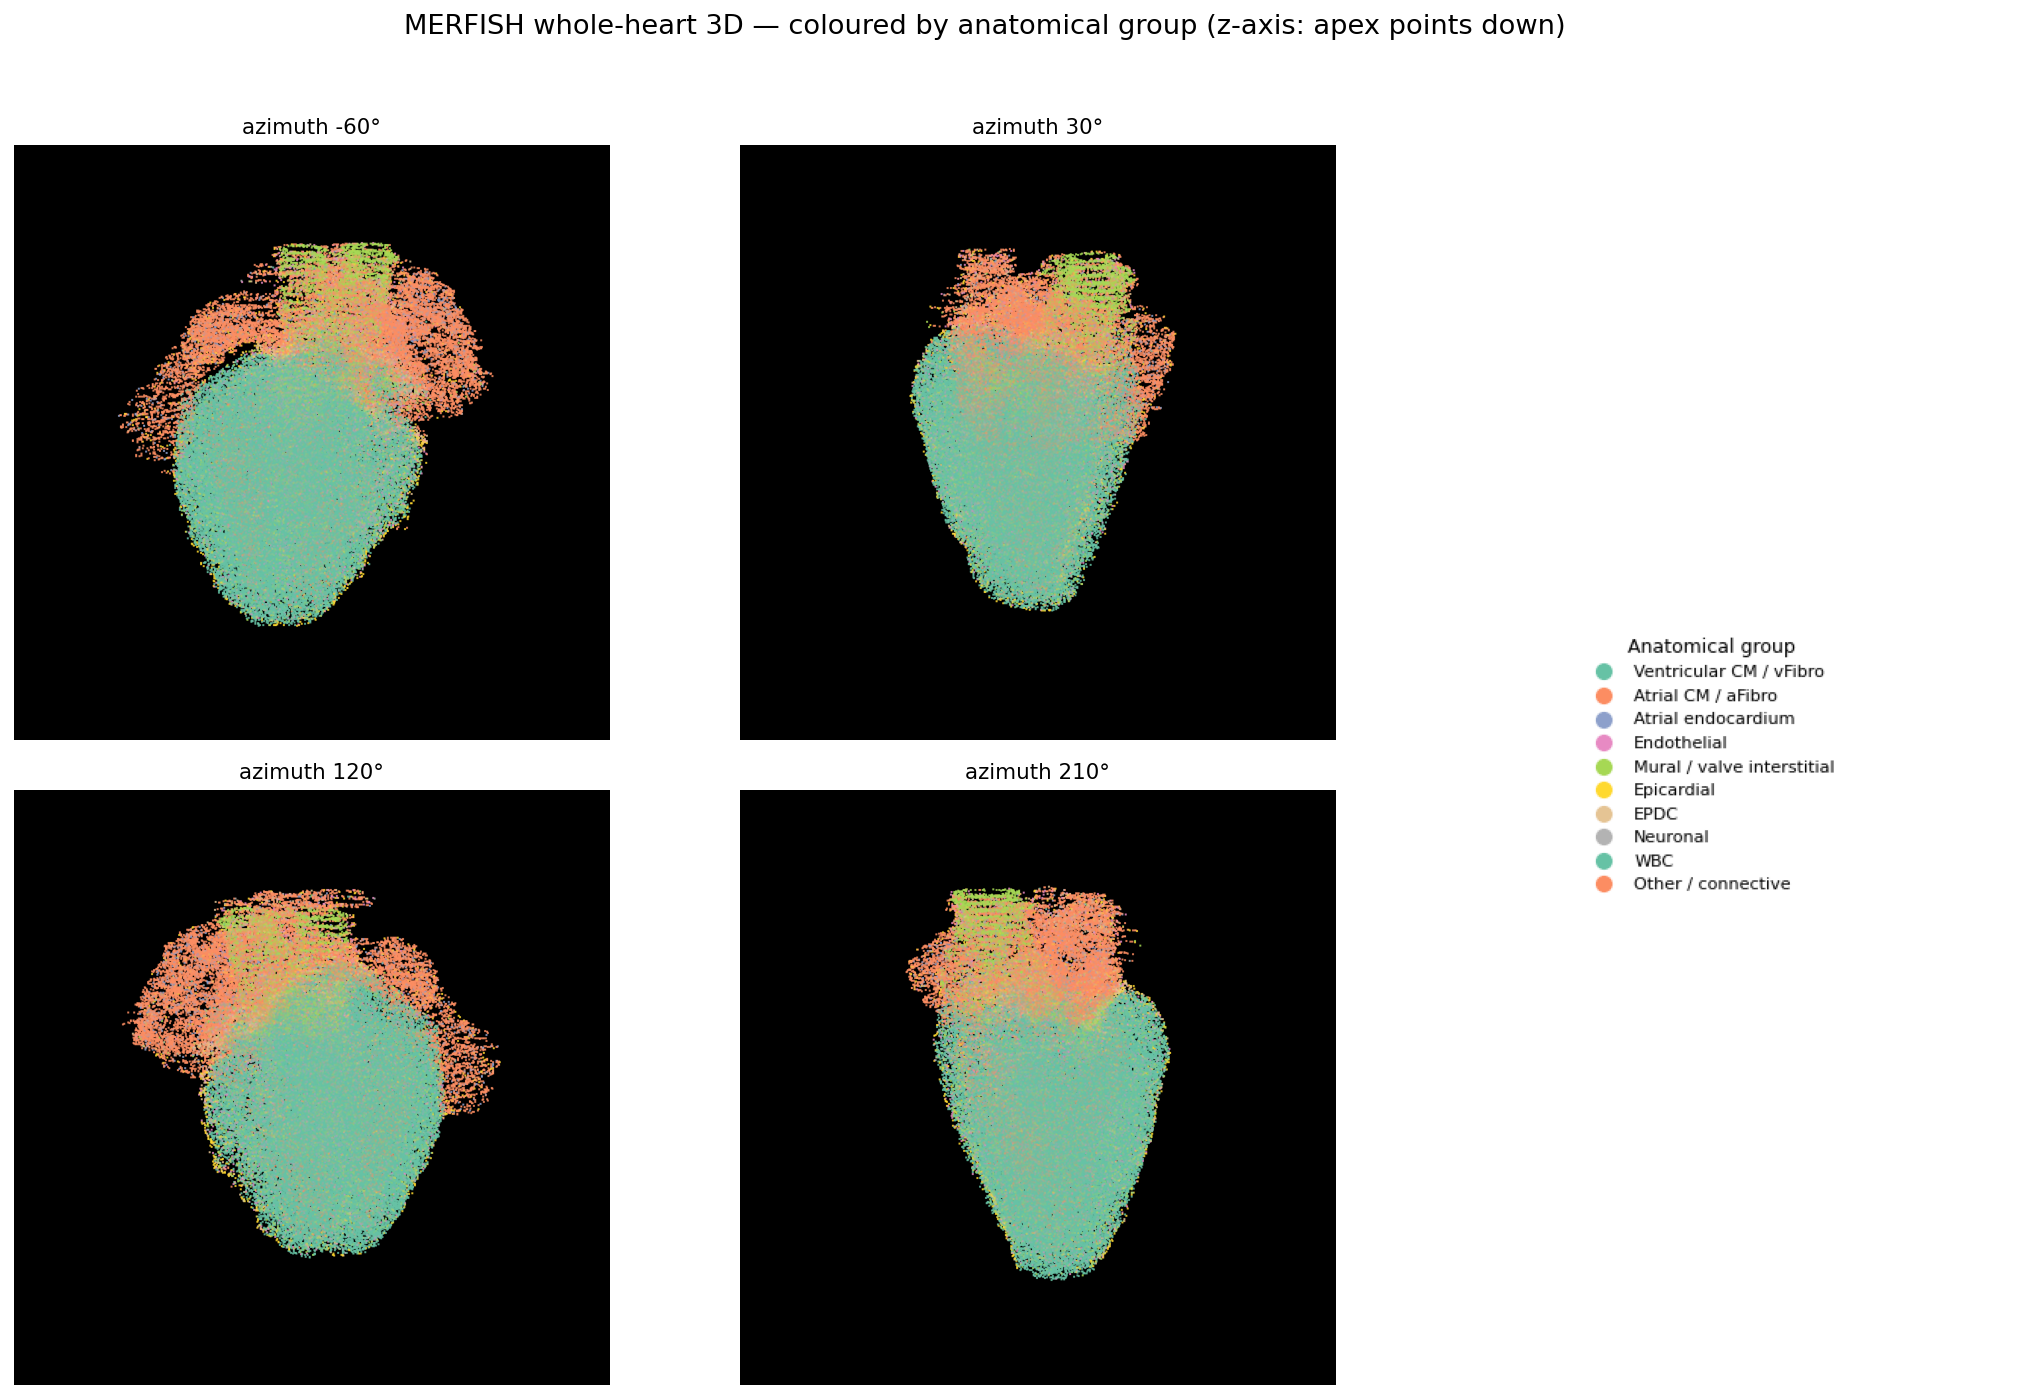
\includegraphics[width=\textwidth]{merfish_3d_chamber.png}
\caption{3D rendering of all 100{,}000 MERFISH cells using the
\(\textsf{X\_spateo\_update}\) embedding (z-axis flipped so the apex
points down), coloured by 10 broad anatomical groups. Four azimuth
viewpoints (\(-60^\circ, 30^\circ, 120^\circ, 210^\circ\)) span the long
axis. The atrial cardiomyocytes (orange) cap the upper pole, the
ventricular cardiomyocytes (teal) form the bulk of the lower body, and
the valve interstitial / mural cell layer (green) demarcates the
atrio-ventricular plane. Fibroblasts and endothelial populations form a
thin envelope on the outer surface and along the chamber linings.}
\label{fig:merfish_3d_chamber}
\end{figure}

\begin{figure}[H]
\centering
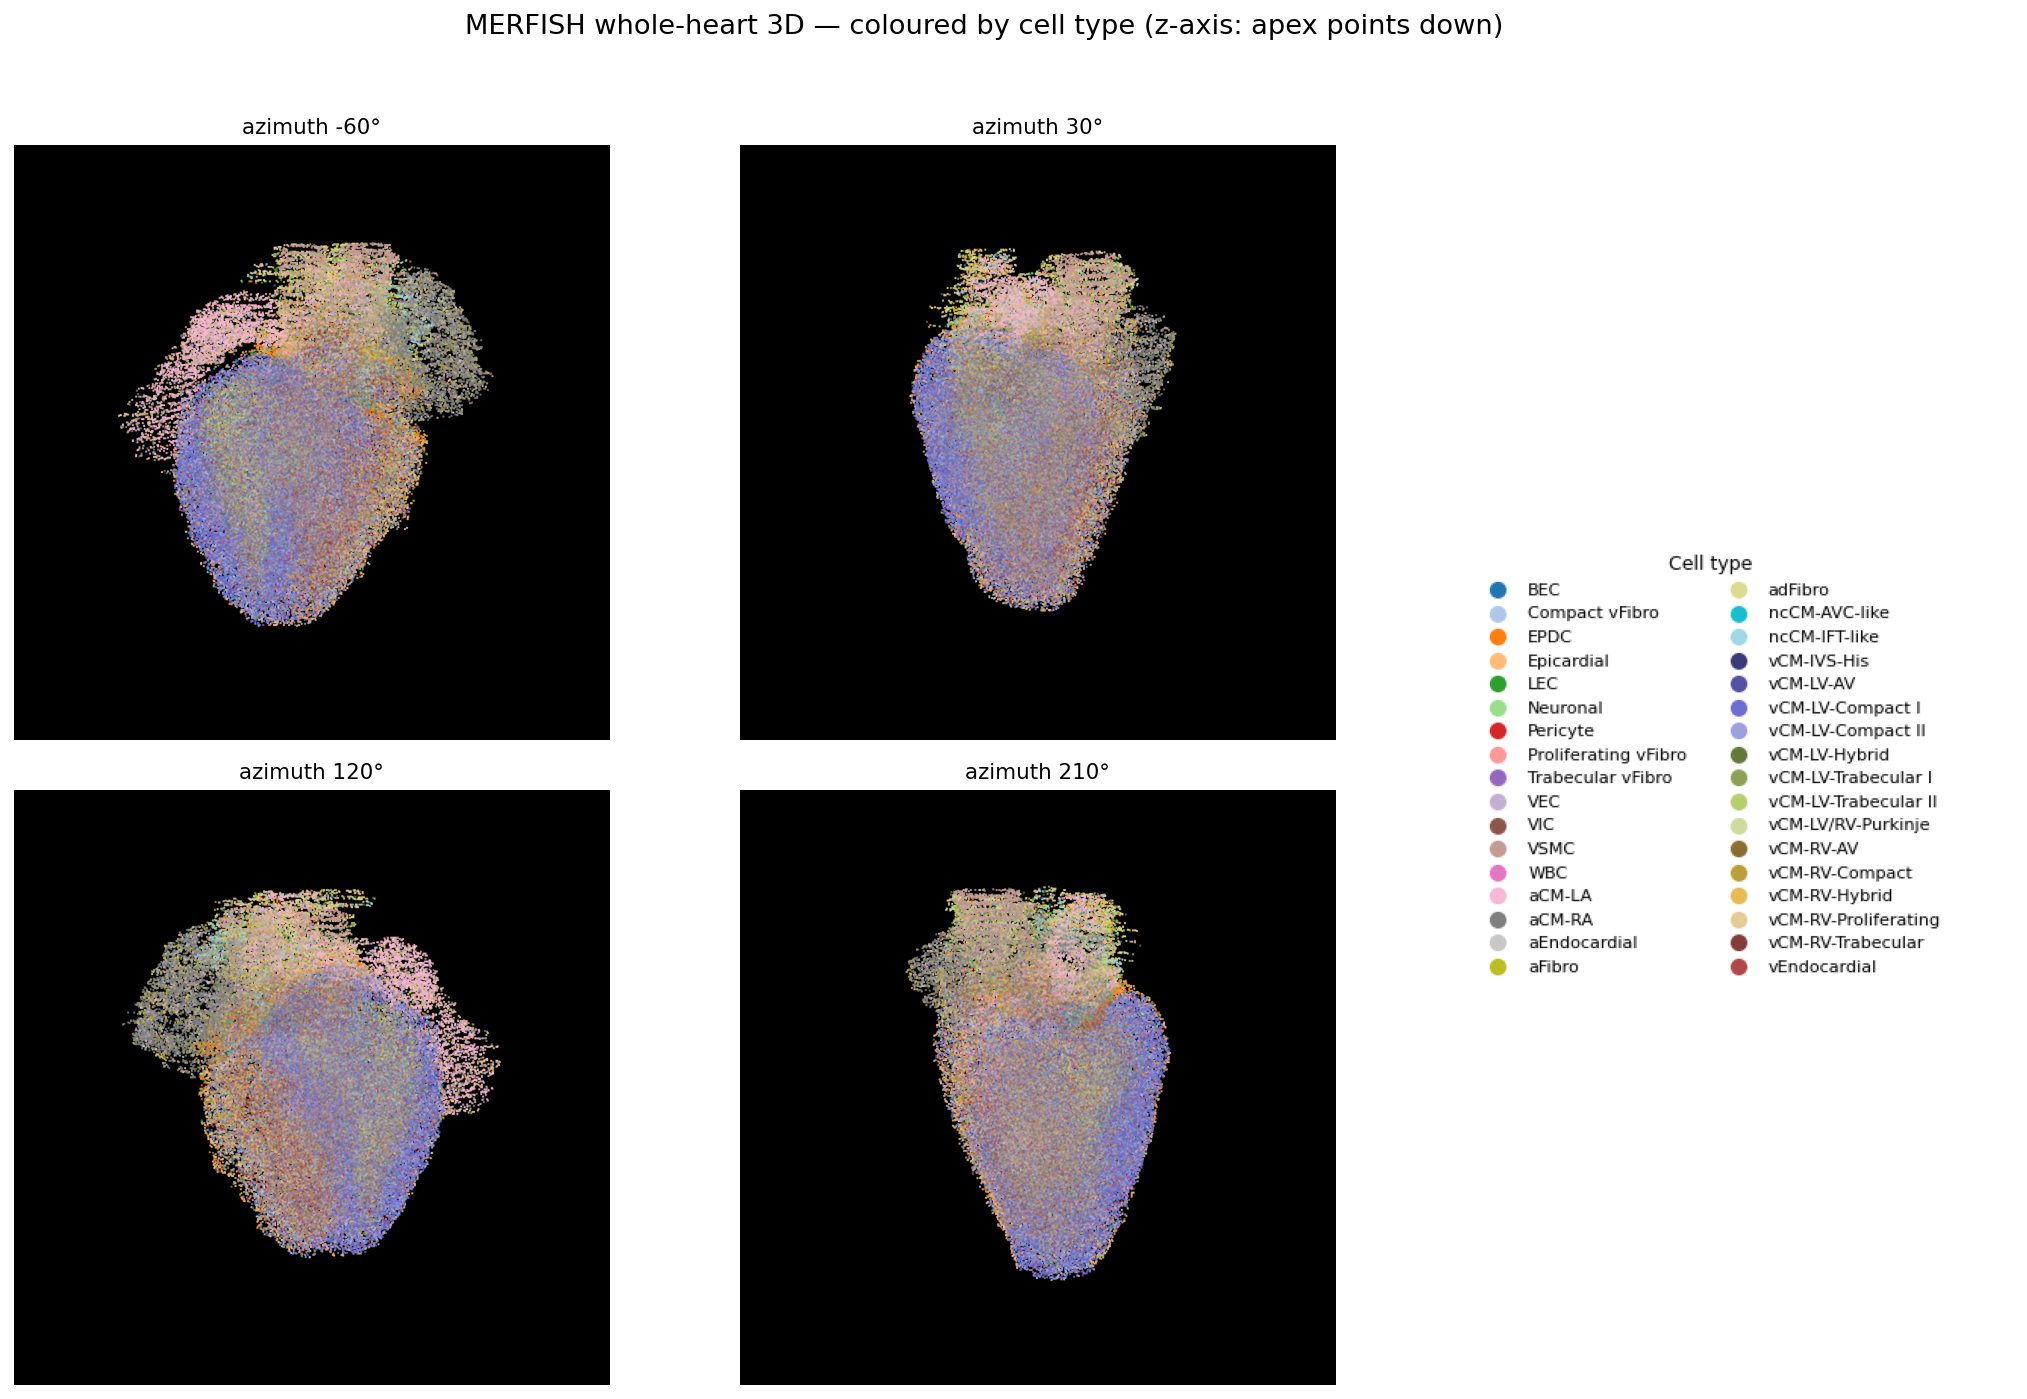
\includegraphics[width=\textwidth]{merfish_3d_celltype.png}
\caption{Same 3D rendering as Fig.~\ref{fig:merfish_3d_chamber} but
coloured by the full 34-class fine annotation. Atrial subtypes
\textsf{aCM-LA} and \textsf{aCM-RA} are visible at the top; the
ventricular wall is dominated by \textsf{vCM-LV-Compact} and
\textsf{vCM-LV-Trabecular}, with right-ventricular and septal
populations on the opposing side; conduction-related populations
(\textsf{vCM-LV/RV-Purkinje}, \textsf{ncCM-AVC-like}, \textsf{ncCM-IFT-like})
occupy focal regions consistent with their expected anatomical niches.
Animated rotations are also available
(\texttt{merfish\_3d\_chamber.gif}, \texttt{merfish\_3d\_celltype.gif}).}
\label{fig:merfish_3d_celltype}
\end{figure}

% ====================================================================
\section{Cross-modality comparison}

\subsection{Broad cell-type composition}

To compare the two modalities on equal footing, the 34 fine MERFISH cell
types were collapsed onto the 11-class broad annotation used by the
scRNA-seq atlas (e.g., \texttt{vCM-LV-Compact I}, \texttt{vCM-RV-Compact}, …
\(\rightarrow\) \texttt{VCM}; \texttt{Compact vFibro}, \texttt{aFibro}, …
\(\rightarrow\) \texttt{FB}). Nine broad classes are shared between the two
datasets: VCM, ACM, FB, MuralCells, Endothelial, Endocardial, Epicardial,
NC, ImmuneCells. Two label families do \emph{not} match exactly:
scRNA-seq distinguishes \textsf{Tz}- from \textsf{Core}-conduction cells,
while MERFISH groups conduction populations differently
(\textsf{vCM-LV/RV-Purkinje}, \textsf{ncCM-IFT-like}, \textsf{ncCM-AVC-like})
— shown as grey labels in Fig.~\ref{fig:crossmod}.

\begin{figure}[H]
\centering
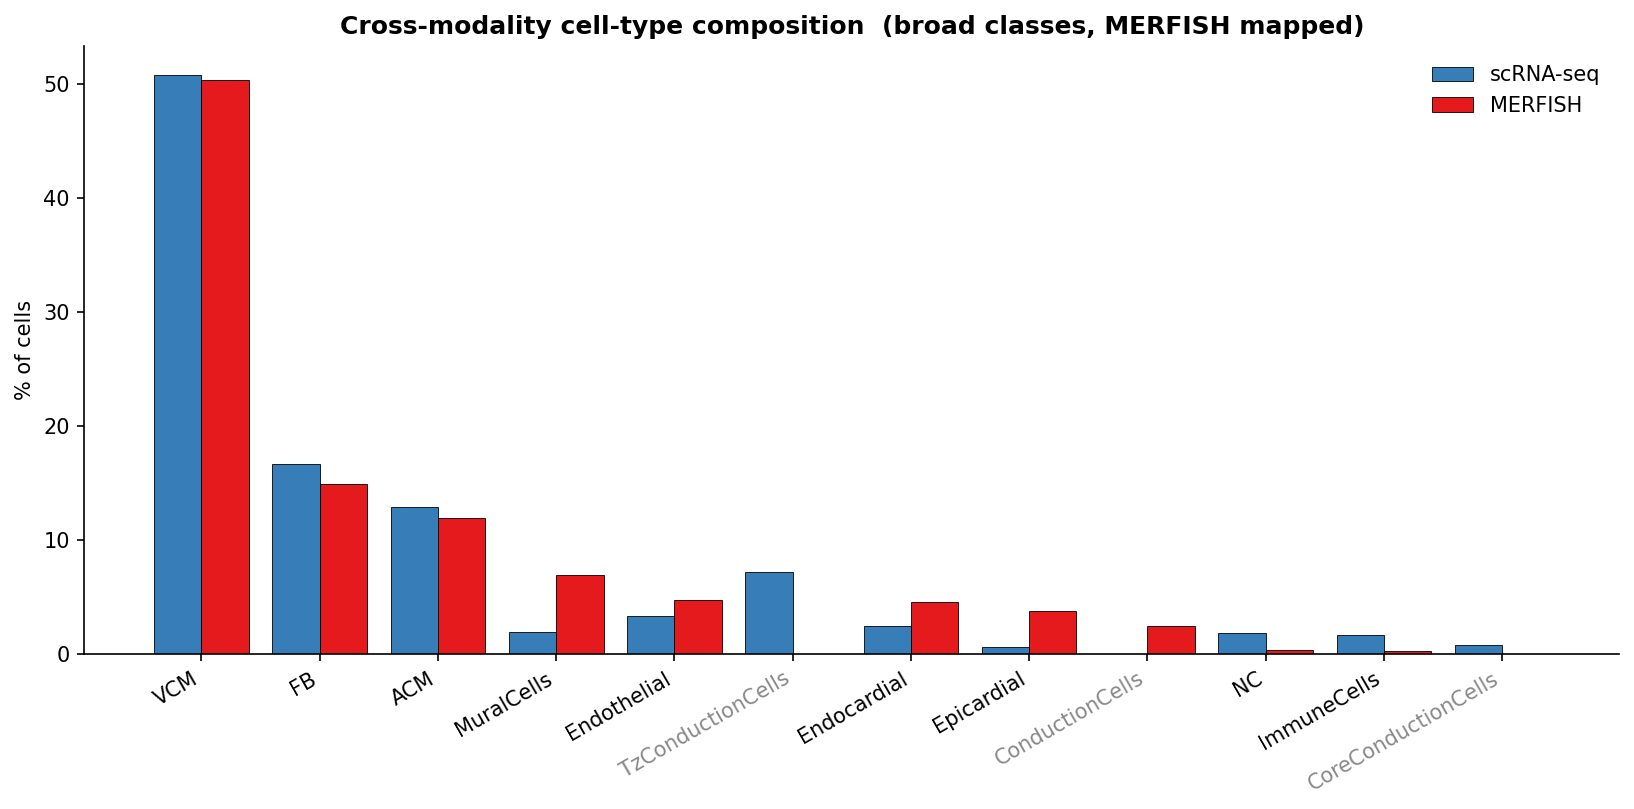
\includegraphics[width=\textwidth]{crossmod_overlap.png}
\caption{Per-modality cell-type fractions for the broad classes. The two
modalities agree closely on the dominant populations: \textbf{VCM} is
\(\sim\)50\% in both, \textbf{FB} 16.6\% vs.\ 14.9\%, and \textbf{ACM}
12.9\% vs.\ 11.9\%. MERFISH over-represents some endothelial and mural
populations relative to scRNA-seq — this is expected because spatial
methods have less drop-out for sparse stromal populations than droplet
scRNA-seq. Greyed labels indicate classes that do not have an exact
counterpart in the other modality due to annotation-scheme differences.}
\label{fig:crossmod}
\end{figure}

\subsection{Joint UMAP}

\begin{figure}[H]
\centering
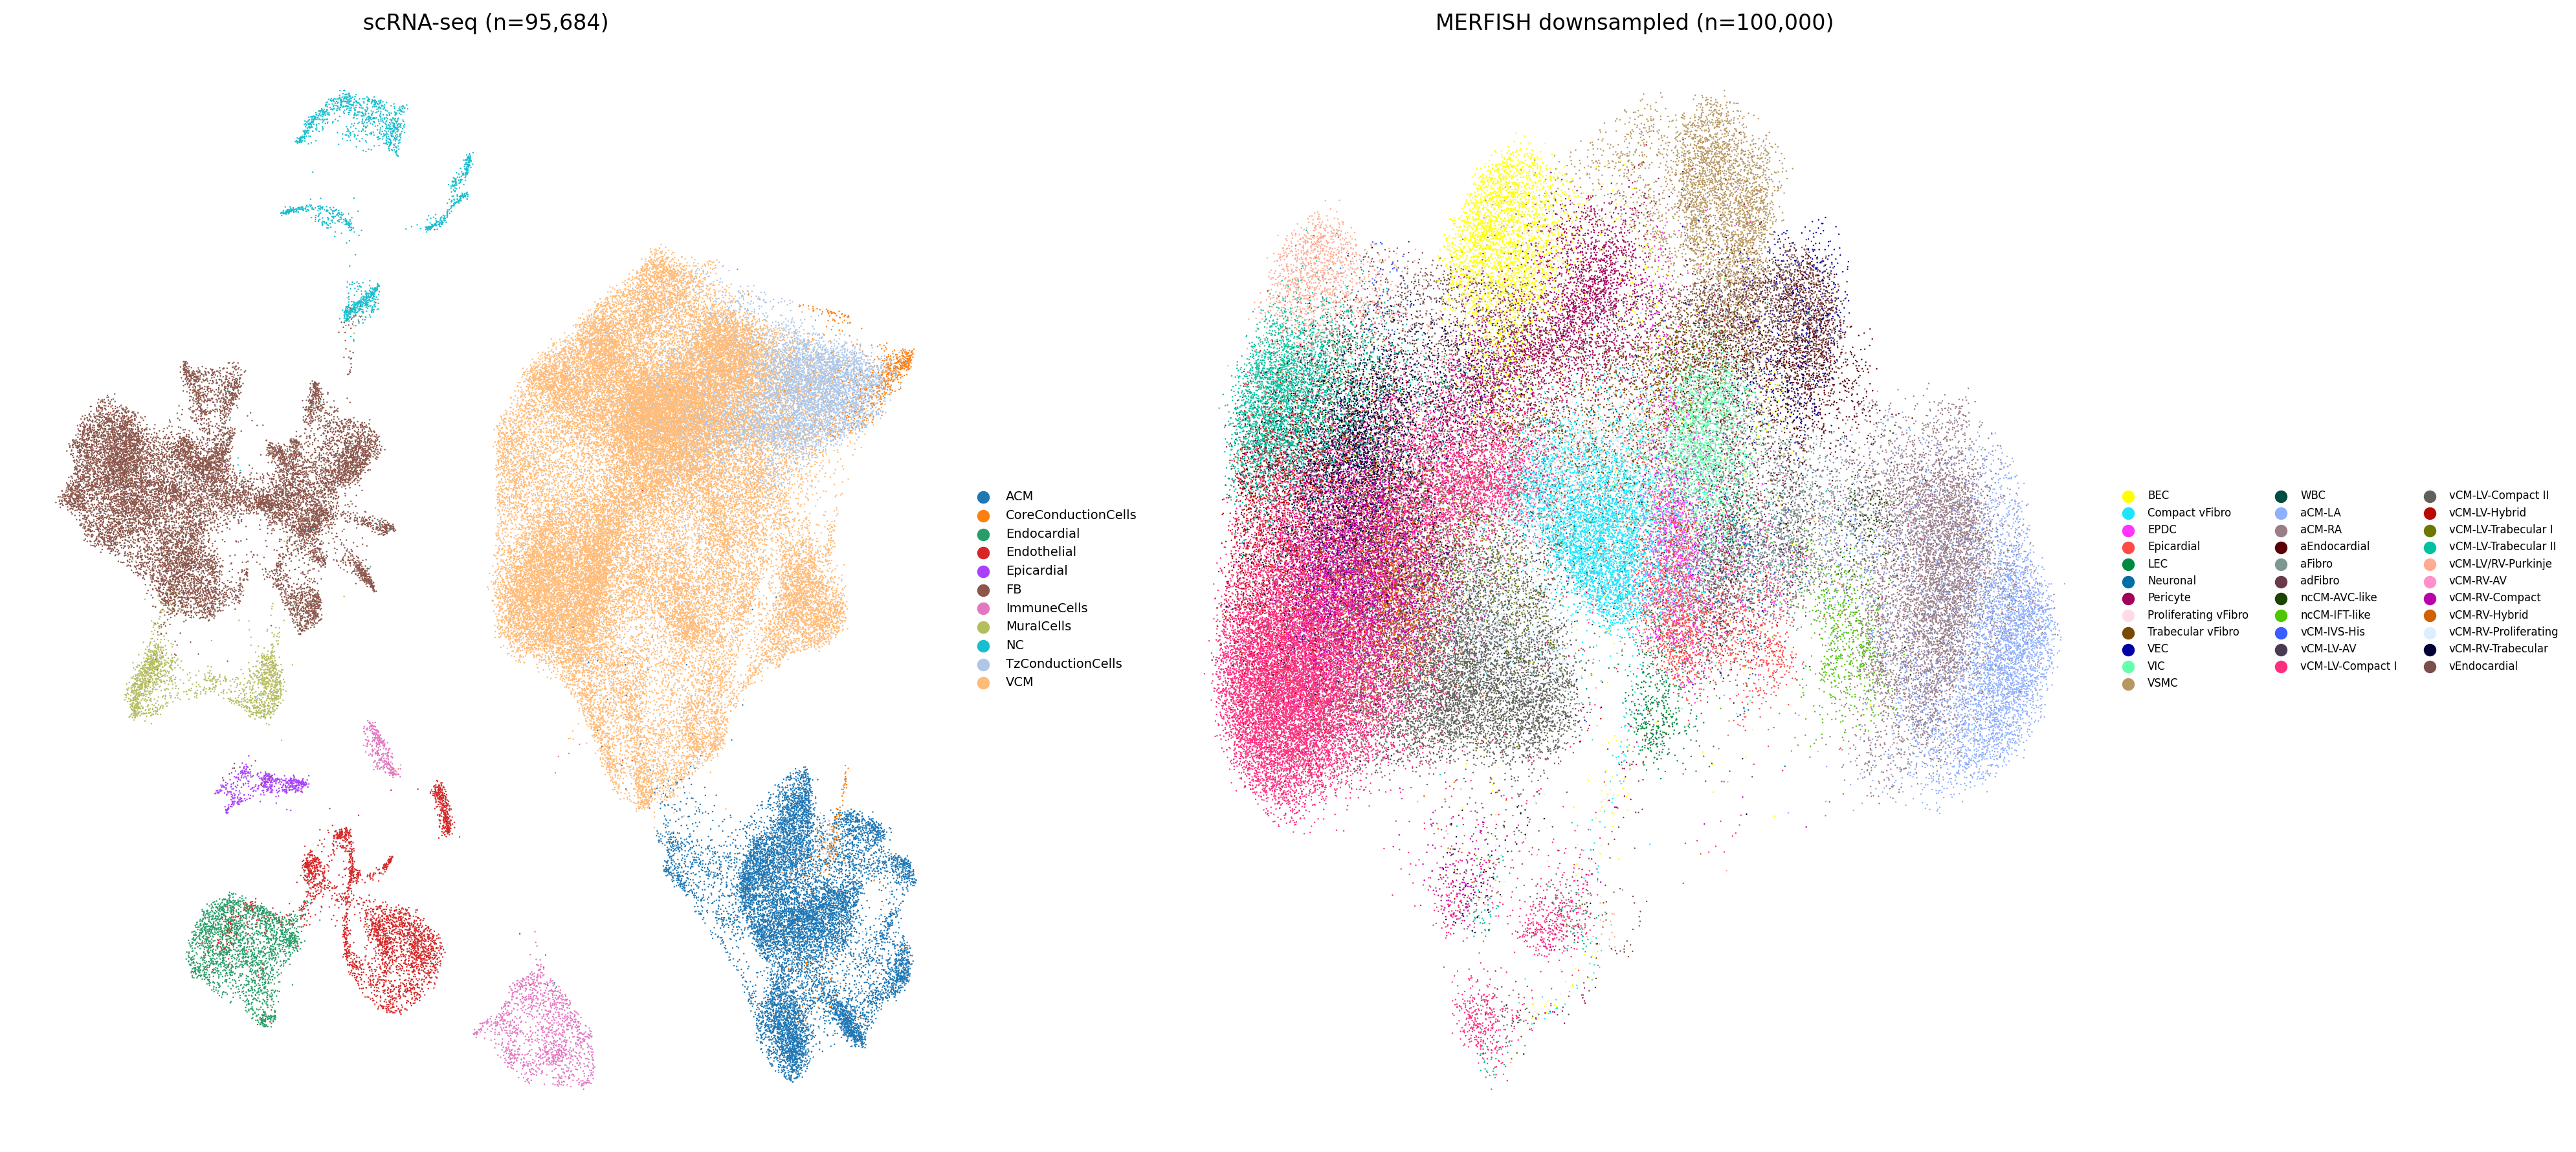
\includegraphics[width=\textwidth]{umap_scrna_vs_merfish.png}
\caption{Side-by-side UMAPs. \textbf{Left:} scRNA-seq UMAP (95{,}684 cells)
computed from the top 3{,}000 highly variable genes (\(\rightarrow\) PCA(50)
\(\rightarrow\) \(k\)NN(15) \(\rightarrow\) UMAP), coloured by the 11
broad classes. \textbf{Right:} the precomputed MERFISH UMAP (100{,}000 cells,
\textsf{X\_umap}) coloured by the 34 fine classes. Both atlases show the
expected dominance of cardiomyocyte clusters with smaller, well-separated
stromal, endothelial, and immune islands.}
\label{fig:umap}
\end{figure}

% ====================================================================
\section{Summary and downstream readiness}

\begin{table}[H]
\centering
\small
\renewcommand{\arraystretch}{1.15}
\begin{tabular}{@{}p{0.40\textwidth} p{0.25\textwidth} p{0.25\textwidth}@{}}
\toprule
\textbf{Metric} & \textbf{scRNA-seq} & \textbf{MERFISH} \\
\midrule
Cells & 95{,}684 & 100{,}000 \\
Genes / panel & 31{,}019 & 238 \\
Median genes / cell & 1{,}375 & 69 \\
Median counts / cell & 2{,}389 & 251 \\
Median \% mitochondrial & 0.41\% & --- \\
Median cell volume & --- & 2.86$\times$10$^{5}$ a.u. \\
Donors / specimens & 8 / 24 samples & 1 / 53 sections \\
PCW span & 11, 12, 13 & 12 \\
Cell-type classes & 11 broad / 111 fine & 34 fine \\
\bottomrule
\end{tabular}
\caption{Per-modality summary statistics.}
\label{tab:summary}
\end{table}

\noindent
The two atlases are complementary: scRNA-seq provides full-transcriptome
coverage across multiple donors and developmental stages, while MERFISH
provides spatial coordinates and cell-type localization within a single
PCW-12 heart. Quality metrics are within standard ranges for both
technologies, batch effects (ATR vs.\ VEN in MERFISH; donor in scRNA-seq)
are modest, and the broad cell-type compositions agree closely. The
nine shared broad classes (VCM, ACM, FB, MuralCells, Endothelial,
Endocardial, Epicardial, NC, ImmuneCells) form the natural anchor for
joint analyses such as MOSCOT optimal-transport mapping
(see \texttt{REPORT.md} for the disease-gene spatial-imputation pipeline
that builds on these data).

\vspace{0.6em}
\noindent\textbf{Reproducibility.}\;\;
Figures generated by
\href{run:scripts/05_data_overview.py}{\texttt{scripts/05\_data\_overview.py}};
metadata snapshot at
\texttt{figures/overview/\_metadata.json};
summary statistics at
\texttt{figures/overview/\_summary\_stats.json}.

\end{document}
